\documentclass[11pt,a4paper]{report}
\usepackage[textwidth=37em,vmargin=30mm]{geometry}
\usepackage{calc,xunicode,amsmath,amssymb,paralist,enumitem,tabu,booktabs,datetime2,xeCJK,xeCJKfntef,listings}
\usepackage{tocloft,fancyhdr,tcolorbox,xcolor,graphicx,eso-pic,xltxtra,xelatexemoji}

\newcommand{\envyear}[0]{2025}
\newcommand{\envdatestr}[0]{2025-09-30}
\newcommand{\envfinaldir}[0]{webdb/2025/20250930/final}

\usepackage[hidelinks]{hyperref}
\hypersetup{
    colorlinks=false,
    pdfpagemode=FullScreen,
    pdftitle={Web Digest - \envdatestr}
}

\setlength{\cftbeforechapskip}{10pt}
\renewcommand{\cftchapfont}{\rmfamily\bfseries\large\raggedright}
\setlength{\cftbeforesecskip}{2pt}
\renewcommand{\cftsecfont}{\sffamily\small\raggedright}

\setdefaultleftmargin{2em}{2em}{1em}{1em}{1em}{1em}

\usepackage{xeCJK,xeCJKfntef}
\xeCJKsetup{PunctStyle=plain,RubberPunctSkip=false,CJKglue=\strut\hskip 0pt plus 0.1em minus 0.05em,CJKecglue=\strut\hskip 0.22em plus 0.2em}
\XeTeXlinebreaklocale "zh"
\XeTeXlinebreakskip = 0pt


\setmainfont{Brygada 1918}
\setromanfont{Brygada 1918}
\setsansfont{IBM Plex Sans}
\setmonofont{JetBrains Mono NL}
\setCJKmainfont{Noto Serif CJK SC}
\setCJKromanfont{Noto Serif CJK SC}
\setCJKsansfont{Noto Sans CJK SC}
\setCJKmonofont{Noto Sans CJK SC}

\setlength{\parindent}{0pt}
\setlength{\parskip}{8pt}
\linespread{1.15}

\lstset{
	basicstyle=\ttfamily\footnotesize,
	numbersep=5pt,
	backgroundcolor=\color{black!5},
	showspaces=false,
	showstringspaces=false,
	showtabs=false,
	tabsize=2,
	captionpos=b,
	breaklines=true,
	breakatwhitespace=true,
	breakautoindent=true,
	linewidth=\textwidth
}






\newcommand{\coverpic}[2]{
    % argv: itemurl, authorname
    Cover photo by #2~~(\href{#1}{#1})
}
\newcommand{\makeheader}[0]{
    \begin{titlepage}
        % \newgeometry{hmargin=15mm,tmargin=21mm,bmargin=12mm}
        \begin{center}
            
            \rmfamily\scshape
            \fontspec{BaskervilleF}
            \fontspec{Old Standard}
            \fontsize{59pt}{70pt}\selectfont
            WEB\hfill DIGEST
            
            \vfill
            % \vskip 30pt
            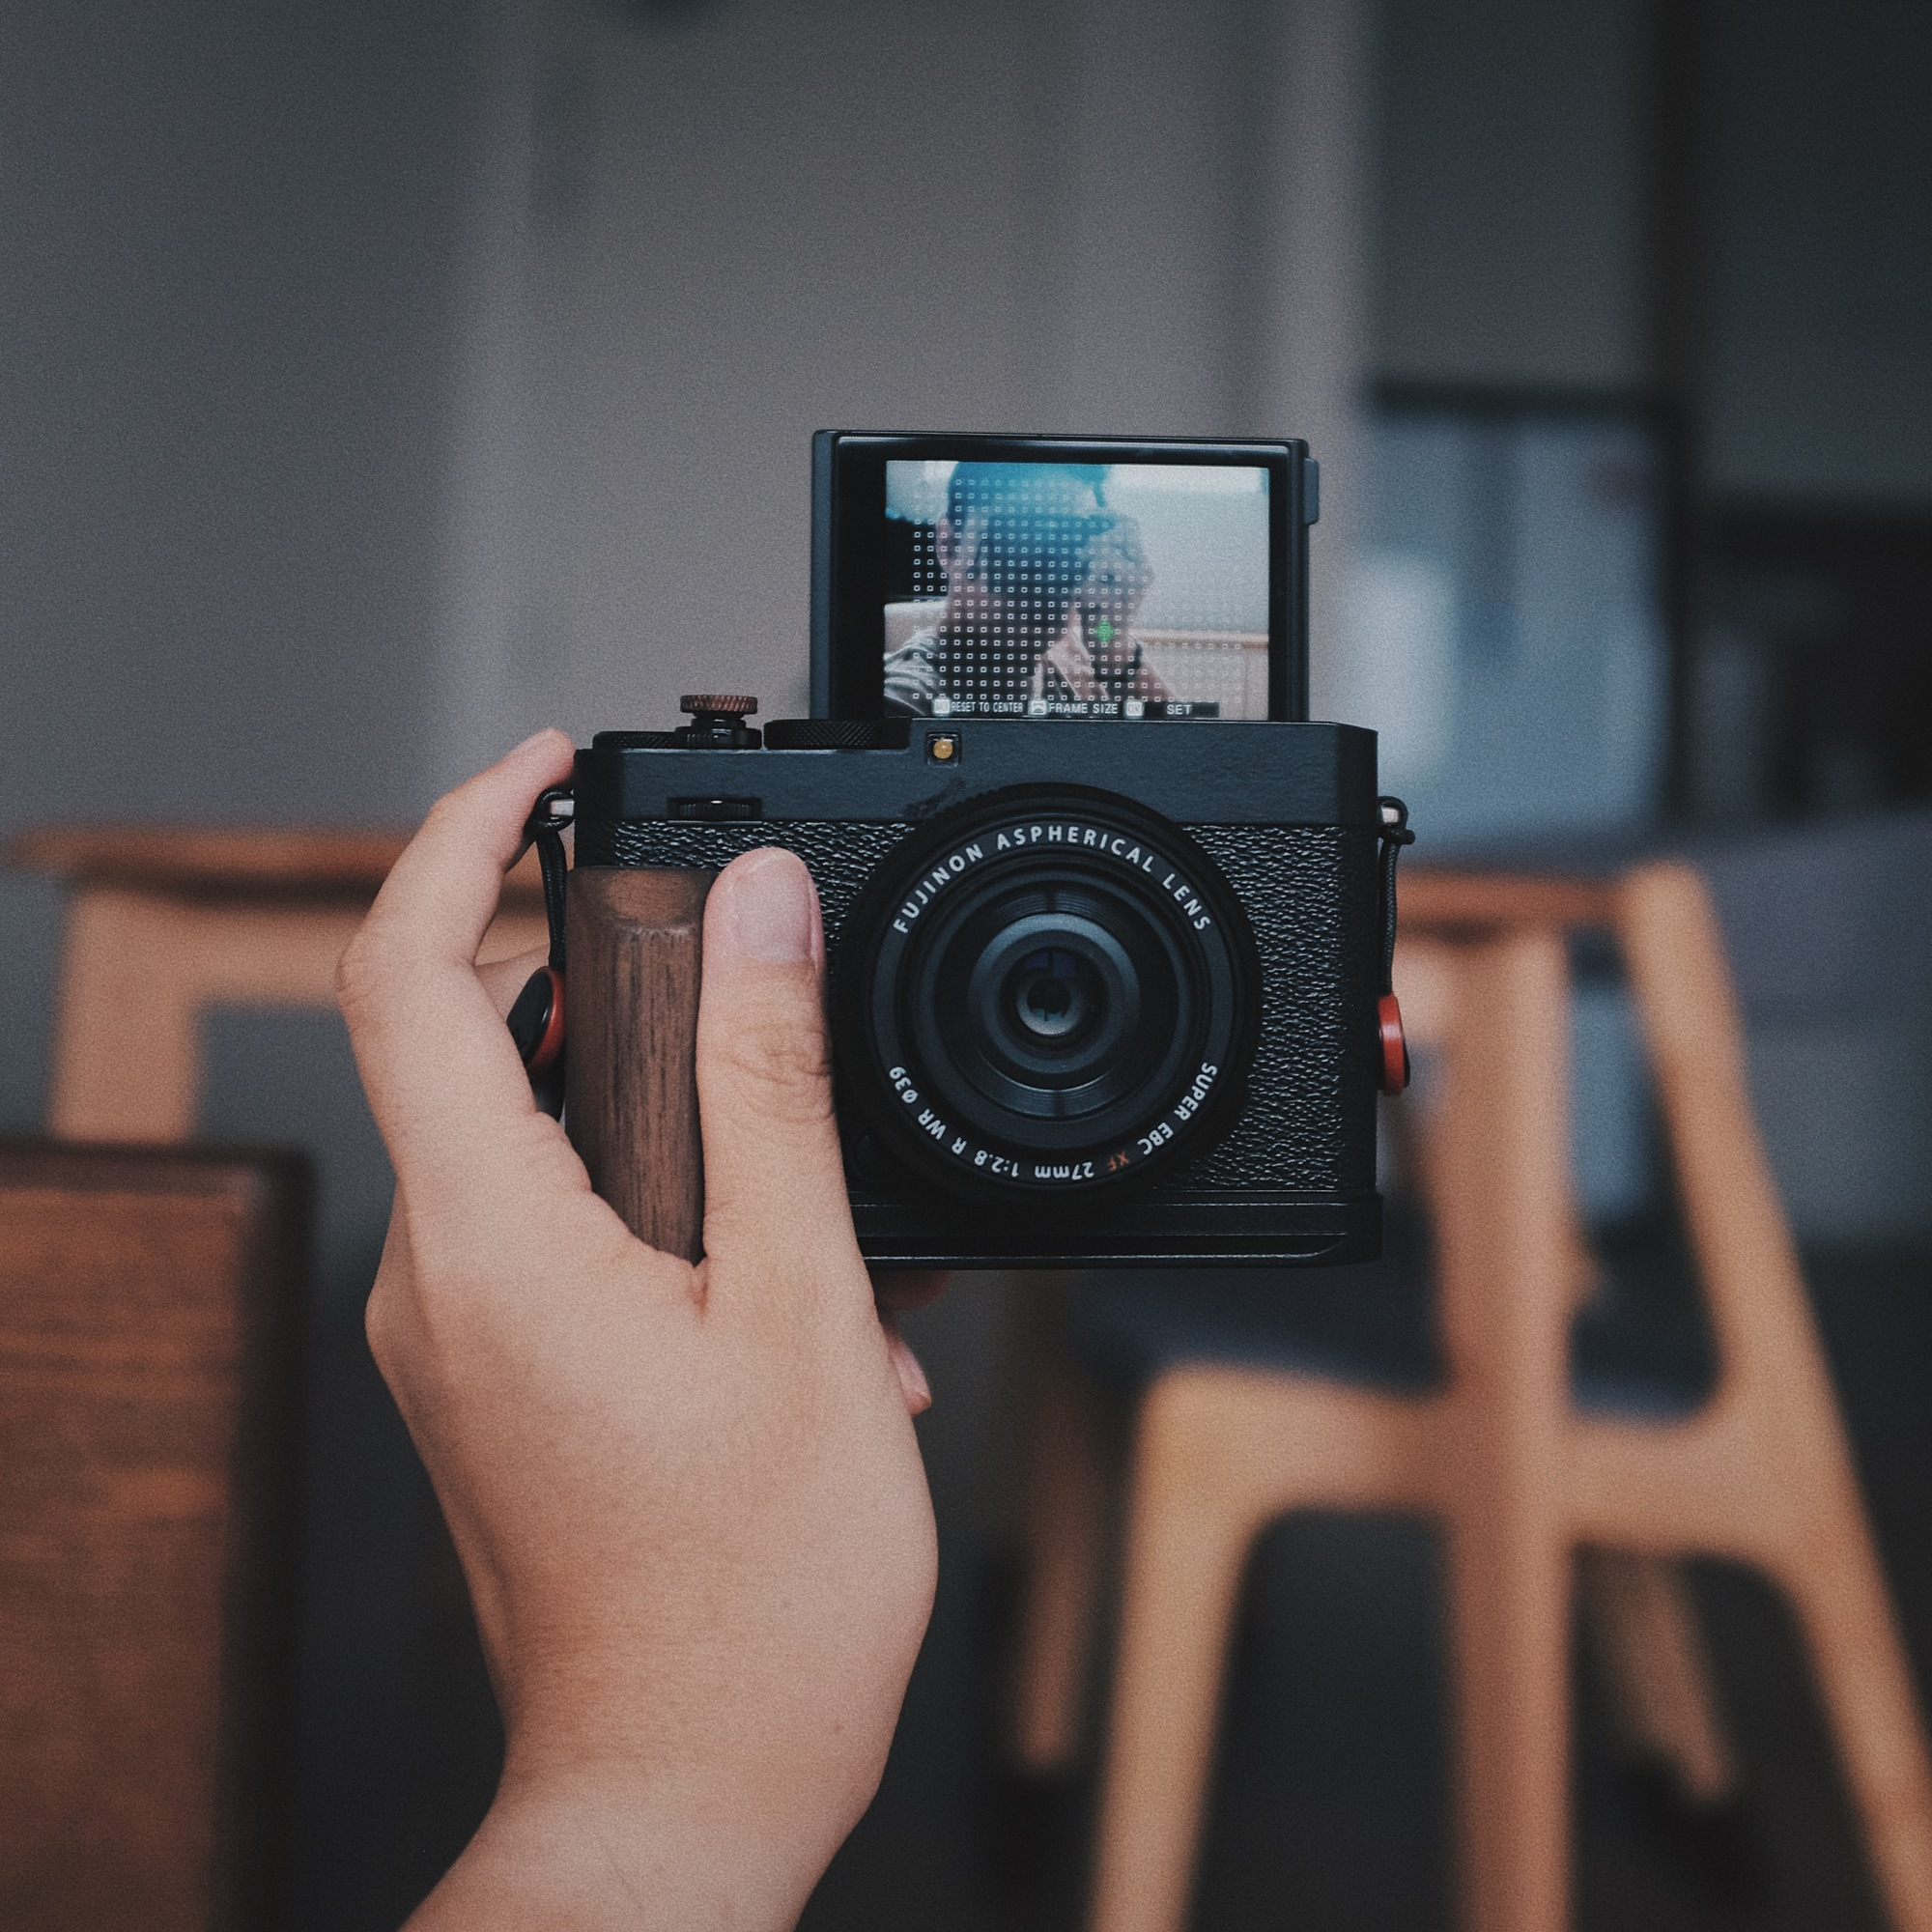
\includegraphics[width=\linewidth]{\envfinaldir/coverpic-prod.jpg}\par
            % \vskip 30pt
            \vfill

            \normalsize\rmfamily\scshape
            \copyright{} The Web Digest Project \hfill\large \envdatestr
        \end{center}
    \end{titlepage}
    % \restoregeometry
}
\newcommand{\simplehref}[1]{%
    \textcolor{blue!80!green}{\href{#1}{#1}}%
}
\renewcommand{\contentsname}{\center\Huge\sffamily\bfseries Contents\par\vskip 20pt}
\newcounter{ipartcounter}
\setcounter{ipartcounter}{0}
\newcommand{\ipart}[1]{
    % \vskip 20pt
    \clearpage
    \stepcounter{ipartcounter}
    \phantomsection
    \addcontentsline{toc}{chapter}{#1}
    % \begin{center}
    %     \Huge
    %     \sffamily\bfseries
    %     #1
    % \end{center}
    % \vskip 20pt plus 7pt
}
\newcounter{ichaptercounter}
\setcounter{ichaptercounter}{0}
\newcommand{\ichapter}[1]{
    % \vskip 20pt
    \clearpage
    \stepcounter{ichaptercounter}
    \phantomsection
    \addcontentsline{toc}{section}{\numberline{\arabic{ichaptercounter}}#1}
    \begin{center}
        \Huge
        \sffamily\bfseries
        #1
    \end{center}
    \vskip 20pt plus 7pt
}
\newcommand{\entrytitlefont}[1]{\subsection*{\raggedright\Large\sffamily\bfseries#1}}
\newcommand{\entryitemGeneric}[2]{
    % argv: title, url
    \parbox{\linewidth}{
        \entrytitlefont{#1}\par\vskip 5pt
        \footnotesize\ttfamily\mdseries
        \simplehref{#2}
    }\vskip 11pt plus 11pt minus 1pt
}
\newcommand{\entryitemGithub}[3]{
    % argv: title, url, desc
    \parbox{\linewidth}{
        \entrytitlefont{#1}\par\vskip 5pt
        \footnotesize\ttfamily\mdseries
        \simplehref{#2}\par\vskip 5pt
        \small\rmfamily\mdseries#3
    }\vskip 11pt plus 11pt minus 1pt
}
\newcommand{\entryitemAp}[3]{
    % argv: title, url, desc
    \parbox{\linewidth}{
        \entrytitlefont{#1}\par\vskip 5pt
        \footnotesize\ttfamily\mdseries
        \simplehref{#2}\par\vskip 5pt
        \small\rmfamily\mdseries#3
    }\vskip 11pt plus 11pt minus 1pt
}
\newcommand{\entryitemHackernews}[3]{
    % argv: title, hnurl, rawurl
    % \parbox{\linewidth}{
    %     \entrytitlefont{#1}\par\vskip 5pt
    %     \footnotesize\ttfamily\mdseries
    %     \simplehref{#3}\par
    %     \textcolor{black!50}{\href{#2}{#2}}
    % }\vskip 11pt plus 11pt minus 1pt
    \begin{minipage}{\linewidth}
            \entrytitlefont{#1}\par\vskip 5pt
            \footnotesize\ttfamily\mdseries
            \simplehref{#3}\par
            \textcolor{black!50}{\href{#2}{#2}}
    \end{minipage}\par\vskip 11pt plus 11pt minus 1pt
}







\begin{document}

\makeheader

\tableofcontents\clearpage




\ipart{Developers}
\ichapter{Hacker News}
\entryitemTwoLinks{California governor signs AI transparency bill into law}{https://news.ycombinator.com/item?id=45418428}{https://www.gov.ca.gov/2025/09/29/governor-newsom-signs-sb-53-advancing-californias-world-leading-artificial-intelligence-industry/}

\entryitemTwoLinks{Remember: Kurt Vonnegut Was 47}{https://news.ycombinator.com/item?id=45418269}{https://www.joanwestenberg.com/p/remember-kurt-vonnegut-was-47}

\entryitemTwoLinks{FCC Accidentally Leaked iPhone Schematics}{https://news.ycombinator.com/item?id=45416231}{https://www.engadget.com/big-tech/fcc-accidentally-leaked-iphone-schematics-potentially-giving-rivals-a-peek-at-company-secrets-154551807.html}

\entryitemTwoLinks{Claude Code 2.0}{https://news.ycombinator.com/item?id=45416228}{https://www.npmjs.com/package/@anthropic-ai/claude-code}

\entryitemTwoLinks{Instant Checkout and the Agentic Commerce Protocol}{https://news.ycombinator.com/item?id=45416080}{https://openai.com/index/buy-it-in-chatgpt/}

\entryitemTwoLinks{Claude Sonnet 4.5}{https://news.ycombinator.com/item?id=45415962}{https://www.anthropic.com/news/claude-sonnet-4-5}

\entryitemTwoLinks{Show HN: Every single torrent is on this website}{https://news.ycombinator.com/item?id=45415539}{https://infohash.lol/}

\entryitemTwoLinks{Write the damn code}{https://news.ycombinator.com/item?id=45415232}{https://antonz.org/write-code/}

\entryitemTwoLinks{Loadmo.re: design inspiration for unconventional web}{https://news.ycombinator.com/item?id=45415207}{https://loadmo.re}

\entryitemTwoLinks{Vertical Solar Panels Are Out Standing}{https://news.ycombinator.com/item?id=45414215}{https://hackaday.com/2025/09/25/vertical-solar-panels-are-out-standing/}

\entryitemTwoLinks{Electronic Arts Goes Private for \$52.5B in Largest LBO}{https://news.ycombinator.com/item?id=45413767}{https://www.wsj.com/business/deals/electronic-arts-to-go-private-in-55-billion-deal-a4a4479c}

\entryitemTwoLinks{Why friction is necessary for growth}{https://news.ycombinator.com/item?id=45413654}{https://jameelur.com/blog/overcoming-friction-leads-to-growth}

\entryitemTwoLinks{Meta-analysis of 2.2M people: Loneliness increases mortality risk by 32\%}{https://news.ycombinator.com/item?id=45413481}{https://lightcapai.medium.com/the-loneliness-epidemic-threatens-physical-health-like-smoking-e063220dde8b}

\entryitemTwoLinks{Larry Ellison – 'citizens will be on their best behavior' amid nonstop recording}{https://news.ycombinator.com/item?id=45413090}{https://fortune.com/2025/09/28/larry-ellison-ai-surveillance-oracle-tiktok-deal-social-media/}

\entryitemTwoLinks{EA Announces Agreement to be Acquired by PIF, Silver Lake, and Affinity Partners}{https://news.ycombinator.com/item?id=45413083}{https://ir.ea.com/press-releases/press-release-details/2025/EA-Announces-Agreement-to-be-Acquired-by-PIF-Silver-Lake-and-Affinity-Partners-for-55-Billion/default.aspx}

\entryitemTwoLinks{What if I don't want videos of my hobby time available to the world?}{https://news.ycombinator.com/item?id=45412419}{https://neilzone.co.uk/2025/09/what-if-i-dont-want-videos-of-my-hobby-time-available-to-the-entire-world/}

\entryitemTwoLinks{DeepSeek-v3.2-Exp}{https://news.ycombinator.com/item?id=45412098}{https://github.com/deepseek-ai/DeepSeek-V3.2-Exp}

\entryitemTwoLinks{Optimizing a 6502 image decoder, from 70 minutes to 1 minute}{https://news.ycombinator.com/item?id=45412022}{https://www.colino.net/wordpress/en/archives/2025/09/28/optimizing-a-6502-image-decoder-from-70-minutes-to-1-minute/}

\entryitemTwoLinks{Google appears to have deleted its political ad archive for the EU}{https://news.ycombinator.com/item?id=45411332}{https://www.thebriefing.ie/google-just-erased-7-years-of-our-political-history/}

\entryitemTwoLinks{What is ``good taste'' in software engineering?}{https://news.ycombinator.com/item?id=45410940}{https://www.seangoedecke.com/taste/}\ichapter{Phoronix}
\entryitemGeneric{\hskip 0pt{}Linus Torvalds Removes The Bcachefs Code From The Linux Kernel}{https://www.phoronix.com/news/Bcachefs-Removed-Linux-6.18}

\entryitemGeneric{\hskip 0pt{}NVIDIA Has Been Supplying NDA'ed Docs To Red Hat For Helping NVK Driver}{https://www.phoronix.com/news/NVK-Vulkan-Red-Hat-NDA-Docs}

\entryitemGeneric{\hskip 0pt{}Linux 6.18 Updating The Baseline For Marking Intel CPU Microcode As Outdated}{https://www.phoronix.com/news/Intel-Old-Microcode-Linux-6.18}

\entryitemGeneric{\hskip 0pt{}Wine 11.0 On Track For January Release With NTSYNC \& New WoW64 Mode}{https://www.phoronix.com/news/Wine-11.0-January-2026}

\entryitemGeneric{\hskip 0pt{}Linux 6.18 Power Management Brings Panther Lake Power Slider \& New Drivers}{https://www.phoronix.com/news/Linux-6.18-Power-Management}

\entryitemGeneric{\hskip 0pt{}NVIDIA, Disney \& Google Contribute Open-Source Newton Engine To The Linux Foundation}{https://www.phoronix.com/news/Linux-Foundation-Newton}

\entryitemGeneric{\hskip 0pt{}Intel Releases New LLM Scaler Betas For GenAI On Battlemage GPUs}{https://www.phoronix.com/news/LLM-Scaler-Betas-EO-Q3}

\entryitemGeneric{\hskip 0pt{}Blender 5.0 Vulkan Render Tests Passing On AMD \& NVIDIA But Failing For Intel}{https://www.phoronix.com/news/Blender-5.0-Vulkan-Intel-Fail}

\entryitemGeneric{\hskip 0pt{}RISC-V With Linux 6.18 Brings Support For MIPS Vendor Extensions}{https://www.phoronix.com/news/Linux-6.18-RISC-V}


\ipart{Developers~~~~(zh-Hans)}
\ichapter{Solidot}
\entryitemGeneric{\hskip 0pt{}流浪行星发现有极光}{https://www.solidot.org/story?sid=82448}

\entryitemGeneric{\hskip 0pt{}瑞士周日公投以微弱多数批准电子身份证}{https://www.solidot.org/story?sid=82447}

\entryitemGeneric{\hskip 0pt{}F-Droid 发表声明反对 Google 验证应用开发者身份的要求}{https://www.solidot.org/story?sid=82446}

\entryitemGeneric{\hskip 0pt{}Linux 6.17 释出}{https://www.solidot.org/story?sid=82444}

\entryitemGeneric{\hskip 0pt{}百万年前的龙人化石或改写人类家谱}{https://www.solidot.org/story?sid=82443}

\entryitemGeneric{\hskip 0pt{}美国考虑要求芯片公司的芯片国内制造和进口各占一半}{https://www.solidot.org/story?sid=82442}

\entryitemGeneric{\hskip 0pt{}研究发现过去 15 年睡眠问题日益严重}{https://www.solidot.org/story?sid=82441}

\entryitemGeneric{\hskip 0pt{}电动汽车公司破产后,车主创建了非盈利组织确保汽车正常运行}{https://www.solidot.org/story?sid=82440}

\entryitemGeneric{\hskip 0pt{}Firefox 将支持图像搜索}{https://www.solidot.org/story?sid=82439}

\entryitemGeneric{\hskip 0pt{}比亚迪超跑时速突破 496 km/h}{https://www.solidot.org/story?sid=82438}

\entryitemGeneric{\hskip 0pt{}Eric Schmidt 呼吁美国科技行业拥抱中国的 996 工作制}{https://www.solidot.org/story?sid=82436}

\entryitemGeneric{\hskip 0pt{}社交纽带的累积效应或有助于健康老龄化}{https://www.solidot.org/story?sid=82435}

\entryitemGeneric{\hskip 0pt{}树莓派推出 Raspberry Pi 500+}{https://www.solidot.org/story?sid=82434}

\entryitemGeneric{\hskip 0pt{}亚马逊 kindle 竭尽所能打击电子书盗版}{https://www.solidot.org/story?sid=82433}

\entryitemGeneric{\hskip 0pt{}yt-dlp 将需要安装 JS 运行时 Deno}{https://www.solidot.org/story?sid=82432}\ichapter{V2EX}
\entryitemGeneric{\hskip 0pt{}[问与答] 非常奇怪的苹果 App 审核失败理由}{https://www.v2ex.com/t/1162771}

\entryitemGeneric{\hskip 0pt{}[问与答] 今天还有上班的吗,感觉上班路上车流量少了一半}{https://www.v2ex.com/t/1162770}

\entryitemGeneric{\hskip 0pt{}[推广] [生日送码]🎉Launchpad 的第三方开源平替软件 Raspberry v0.0.15 稳定版,全免 Pro 激活码+半折优惠码!}{https://www.v2ex.com/t/1162769}

\entryitemGeneric{\hskip 0pt{}[投资] 2024 年社保投资收益率 8.1\%}{https://www.v2ex.com/t/1162768}

\entryitemGeneric{\hskip 0pt{}[酷工作] [深圳][Lime]招聘高级 IT 工程师}{https://www.v2ex.com/t/1162767}

\entryitemGeneric{\hskip 0pt{}[健康] 右手食指商阳穴常年灼热, 催动指甲异常生长, 求调理之法}{https://www.v2ex.com/t/1162766}

\entryitemGeneric{\hskip 0pt{}[硬件] 这个配置怎样}{https://www.v2ex.com/t/1162765}

\entryitemGeneric{\hskip 0pt{}[问与答] 请问,微信门口常驻的特警车是干啥的?}{https://www.v2ex.com/t/1162764}

\entryitemGeneric{\hskip 0pt{}[程序员] 现在哪个 window 笔记本能实现和 mac 一样合盖休眠零掉电,开盖即用功能?}{https://www.v2ex.com/t/1162761}

\entryitemGeneric{\hskip 0pt{}[生活] 夫妻两人在国外生活,担心孩子教育问题,值不值得为了孩子回国}{https://www.v2ex.com/t/1162760}

\entryitemGeneric{\hskip 0pt{}[问与答] 小红书刷到的 macmini4 集群视频是干嘛的}{https://www.v2ex.com/t/1162758}

\entryitemGeneric{\hskip 0pt{}[OpenAI] 有哪些 ChatGPT Pulse 的开源替代?}{https://www.v2ex.com/t/1162757}

\entryitemGeneric{\hskip 0pt{}[English] 如何通过自学实现无字幕听懂美剧:我的 4000 小时英语自学经历}{https://www.v2ex.com/t/1162756}

\entryitemGeneric{\hskip 0pt{}[分享发现] 从发现:只要开着代理,即便设置了 DIRECT 规则,阿里云中国站也会被重定向到国际站 之后联想到的}{https://www.v2ex.com/t/1162755}

\entryitemGeneric{\hskip 0pt{}[分享创造] [分享] 国庆自驾必备!做了个 YouTube 转播客的工具,长途开车不无聊}{https://www.v2ex.com/t/1162754}

\entryitemGeneric{\hskip 0pt{}[分享创造] NanoPhoto.AI,现在推出还来得及吗?无需提示词即可玩转 NanoBanana}{https://www.v2ex.com/t/1162752}

\entryitemGeneric{\hskip 0pt{}[加密货币] 英国警方查获钱志敏 6 万枚比特币价值 480 亿,这案子赚大发了}{https://www.v2ex.com/t/1162750}

\entryitemGeneric{\hskip 0pt{}[Linux] 需要买一个 16 寸国产笔记本,听听各位的建议}{https://www.v2ex.com/t/1162749}

\entryitemGeneric{\hskip 0pt{}[分享发现] OMG 的神奇威力!}{https://www.v2ex.com/t/1162748}

\entryitemGeneric{\hskip 0pt{}[酷工作] [上海] AI 创作社区 Startup 招 iOS 工程师}{https://www.v2ex.com/t/1162746}

\entryitemGeneric{\hskip 0pt{}[远程工作] 招聘<远程>Spine 动画师}{https://www.v2ex.com/t/1162745}

\entryitemGeneric{\hskip 0pt{}[Apple] iPhone 17 系列展示机``划痕''的成因及解决的神奇妙妙配方}{https://www.v2ex.com/t/1162744}

\entryitemGeneric{\hskip 0pt{}[Linux] Beyond Compare 在 Linux 平台上有办法禁用光标闪烁吗?}{https://www.v2ex.com/t/1162741}

\entryitemGeneric{\hskip 0pt{}[远程工作] YesNoMarket 诚聘技术人才(远程办公)}{https://www.v2ex.com/t/1162739}

\entryitemGeneric{\hskip 0pt{}[问与答] 有没有可以自动给人脸/人物分组的 windows 相册应用呢}{https://www.v2ex.com/t/1162738}

\entryitemGeneric{\hskip 0pt{}[硬件] 2025 10 月组装电脑}{https://www.v2ex.com/t/1162737}

\entryitemGeneric{\hskip 0pt{}[分享创造] 一个开源的电子礼簿系统}{https://www.v2ex.com/t/1162736}

\entryitemGeneric{\hskip 0pt{}[分享创造] 用一句话, AI 写出一个故事}{https://www.v2ex.com/t/1162735}

\entryitemGeneric{\hskip 0pt{}[问与答] 问下,真的有人不知道什么是 vibe coding 么?}{https://www.v2ex.com/t/1162734}

\entryitemGeneric{\hskip 0pt{}[分享创造] The Book Of Answers}{https://www.v2ex.com/t/1162733}

\entryitemGeneric{\hskip 0pt{}[问与答] 最近 github 搜索总是超时}{https://www.v2ex.com/t/1162731}

\entryitemGeneric{\hskip 0pt{}[跑步] 2026 香港马拉松中签啦}{https://www.v2ex.com/t/1162730}

\entryitemGeneric{\hskip 0pt{}[投资] v 站股友交流群}{https://www.v2ex.com/t/1162727}

\entryitemGeneric{\hskip 0pt{}[iPhone] iPhone 11 升级 IOS 26 超级丝滑.}{https://www.v2ex.com/t/1162725}

\entryitemGeneric{\hskip 0pt{}[香港] 香港复星国际证券 ,内地身份还可以开通。}{https://www.v2ex.com/t/1162724}

\entryitemGeneric{\hskip 0pt{}[问与答] 求推荐适合家用的 ac+ap 设备}{https://www.v2ex.com/t/1162723}

\entryitemGeneric{\hskip 0pt{}[iPhone] 17pm 购买}{https://www.v2ex.com/t/1162722}

\entryitemGeneric{\hskip 0pt{}[问与答] 每次临近长假都有帖子问,大家准备去哪玩。}{https://www.v2ex.com/t/1162721}

\entryitemGeneric{\hskip 0pt{}[问与答] 大路灯,大家有推荐的吗?}{https://www.v2ex.com/t/1162720}

\entryitemGeneric{\hskip 0pt{}[PRO] 建议:广告预览提供真实尺寸}{https://www.v2ex.com/t/1162719}

\entryitemGeneric{\hskip 0pt{}[OpenAI] GPT 4o 准备教会我, GPT 5 感觉要送走我}{https://www.v2ex.com/t/1162718}

\entryitemGeneric{\hskip 0pt{}[微信] 喜当爹? 如何删除微信好友里的 学校通知 这个机器人}{https://www.v2ex.com/t/1162717}

\entryitemGeneric{\hskip 0pt{}[程序员] Cursor userdashboard 跳舞闪烁一天了}{https://www.v2ex.com/t/1162716}

\entryitemGeneric{\hskip 0pt{}[加密货币] Bitcoin dominance 即将跌破 58\%,山寨季来了。}{https://www.v2ex.com/t/1162715}

\entryitemGeneric{\hskip 0pt{}[创业组队] 找几个志同道合的朋友,聊聊创业想法}{https://www.v2ex.com/t/1162713}

\entryitemGeneric{\hskip 0pt{}[问与答] [不懂就问] 想开发一个自用的中医诊所软件,需要学习什么,用什么语言比较好}{https://www.v2ex.com/t/1162712}

\entryitemGeneric{\hskip 0pt{}[职场话题] 从身边的角度告诉大家现在有多不景气}{https://www.v2ex.com/t/1162711}

\entryitemGeneric{\hskip 0pt{}[问与答] 马斯克赶紧把手机造出来}{https://www.v2ex.com/t/1162710}

\entryitemGeneric{\hskip 0pt{}[问与答] 盛世山河添喜色,良宵明月伴归途——双节大家去哪玩?}{https://www.v2ex.com/t/1162708}

\entryitemGeneric{\hskip 0pt{}[问与答] 为什么会有 0.18 铜币}{https://www.v2ex.com/t/1162707}


\ipart{Generic News}







\clearpage
\leavevmode\vfill
\footnotesize

Copyright \copyright{} 2023-2025 Neruthes and other contributors.

This document is published with CC BY-NC-ND 4.0 license.

The entries listed in this newsletter may be copyrighted by their respective creators.

This newsletter is generated by the Web Digest project.

The newsletters are also delivered via Telegram channel \CJKunderline{\href{https://t.me/webdigestchannel}{https://t.me/webdigestchannel}}.\\
RSS feed is available at \CJKunderline{\href{https://webdigest.pages.dev/rss.xml}{https://webdigest.pages.dev/rss.xml}}.

This newsletter is available in PDF at
\CJKunderline{\href{https://webdigest.pages.dev/}{https://webdigest.pages.dev/}}.

The source code being used to generate this newsletter is available at\\
\CJKunderline{\href{https://github.com/neruthes/webdigest}{https://github.com/neruthes/webdigest}}.

This newsletter is also available in
\CJKunderline{\href{http://webdigest.pages.dev/readhtml/\envyear/WebDigest-20250930.html}{HTML}} and
\CJKunderline{\href{https://github.com/neruthes/webdigest/blob/master/markdown/\envyear/WebDigest-20250930.md}{Markdown}}.


\coverpic{https://unsplash.com/photos/man-wearing-aviator-sunglasses-across-city-building-tPWHTBzQVIM}{roland deason}


\end{document}
